\documentclass{bmstu}

\usepackage{pdfpages}

\addbibresource{inc/biblio/sources.bib}

\begin{document}

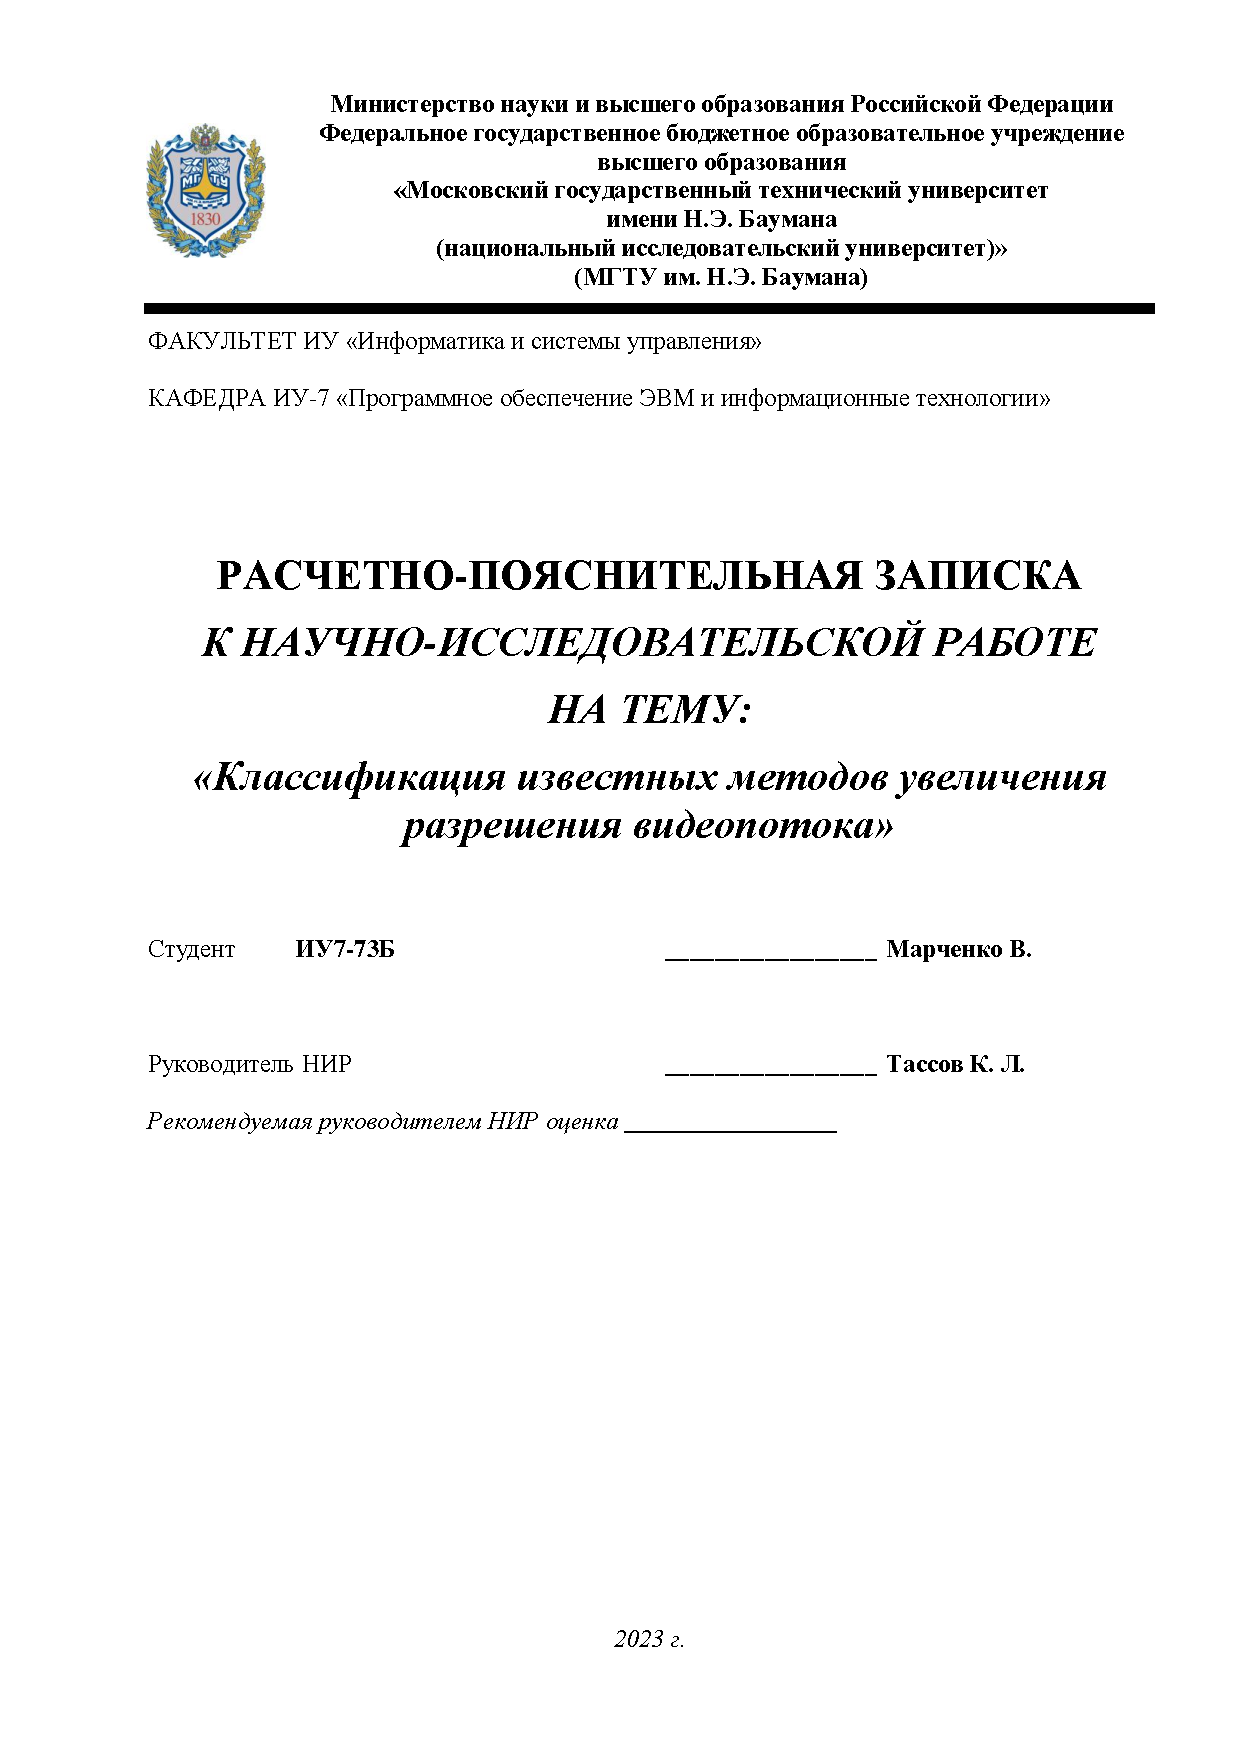
\includepdf[pages=-]{inc/img/title.pdf}

\setcounter{page}{3}

{\centering \chapter*{РЕФЕРАТ}}

Отчет X с., X рис., X табл., X источн., X прил.

\noindent ВИДЕО, ВИДЕОПОТОК, ВИДЕОИЗОБРАЖЕНИЕ, РАЗРЕШЕНИЕ, ПРЕОБРАЗОВАНИЕ ФУРЬЕ, НЕЙРОННЫЕ СЕТИ

Объектом исследования являются методы увеличения разрешения видеопотока.

Цель работы: классификация известных методов увеличения разрешения видеопотока.

В результате исследования было проведено сравнение ... по ... критериям.

Область применения результатов --- ...

Результат работы...

\maketableofcontents

{\centering \chapter*{ПЕРЕЧЕНЬ СОКРАЩЕНИЙ И ОБОЗНАЧЕНИЙ}}

В настоящем отчете о НИР применяют следующие сокращения и обозначения:

\begin{table}[H]
\begin{tabular}{p{3cm}p{13.5cm}}
VSR & Суперразрешение видео (Video Super-Resolution)
\tabularnewline
SISR & Суперразрешение фото (Single-Image Super-Resolution)
\tabularnewline
DFT & Дискретное преобразование Фурье (Discrete Fourier Transform)
\tabularnewline
DCT & Дискретное косинусное преобразование (Discrete Cosine Transform)
\tabularnewline
DWT & Дискретное вейвлет-преобразование (Discrete Wavelet Transform)
\tabularnewline
NEDI & New Edge-Directed Interpolation
\tabularnewline
GBA & Grouped Bees Algorithm
\tabularnewline
POCS & Проецирование в выпуклые множества (Projections onto Convex Sets)
\tabularnewline
IBP & Interval Bound Interpolation
\tabularnewline
RLS & Рекуррентный метод наименьших квадратов (Recursive Least Squares)
\tabularnewline
MAP & Оценка апостериорного максимума (Maximum a posteriori Probability)
\tabularnewline
MLE & Метод максимального правдоподобия (Maximum Likelihood Estimation)
\tabularnewline
MRF & Марковское случайное поле (Markov Random Field)
\tabularnewline
\end{tabular}
\end{table}

{\centering \chapter*{ВВЕДЕНИЕ}}
\addcontentsline{toc}{chapter}{ВВЕДЕНИЕ}

Суперразрешение --- это способ получения изображения или видеоизображения с высоким разрешением из изображений с низким разрешением~\cite{Park2003}. 
В отличие от суперразрешения одного изображения (SISR), основная цель суперразрешения видео --- не только восстановить больше мелких деталей при сохранении крупных, но и сохранить согласованность движения.

Во многих областях, работающих с видео, люди имеют дело с различными типами деградации видео, включая понижение разрешения. 
Разрешение видео может снизиться из-за несовершенства измерительных устройств. 
Плохое освещение и погодные условия добавляют шум. 
Движение объектов и камеры также ухудшает качество видео. 
Методы суперразрешения помогают восстановить исходное видео. 
Это полезно в широком спектре приложений, таких как~\cite{Daithankar2021}:
\begin{enumerate}
\item[1)] видеонаблюдение (для улучшения качества видео, снятого с камеры, а также распознавания номеров автомобилей и лиц);
\item[2)] медицинская визуализация (чтобы лучше обнаружить некоторые органы или ткани для клинического анализа и медицинского вмешательства);
\item[3)] судебно-медицинская экспертиза (для помощи в расследовании в ходе уголовного процесса);
\item[4)] астрономия (для улучшения качества видео звезд и планет);
\item[5)] дистанционное зондирование (для облегчения наблюдения за объектом);
\item[6)] микроскопия (для усиления возможностей микроскопов).
\end{enumerate}

Суперразрешение видео также помогает решить задачу обнаружения объектов, распознавания лиц и символов (в качестве этапа предварительной обработки).

Существует множество подходов к решению этой задачи, но она по-прежнему остается популярной и сложной.

Цель научно-исследовательской работы: провести обзор известных методов увеличения разрешения видеопотока и классифицировать их по сформулированным критериям.

Задачи научно-исследовательской работы:
\begin{enumerate}
\item[1)] исследовать предметную область увеличения разрешения видеопотока;
\item[2)] проанализировать известные методы увеличения разрешения видеопотока;
\item[3)] сформулировать критерии для сравнения этих методов;
\item[4)] сравнить методы увеличения разрешения видеопотока по сформулированным критериям.
\end{enumerate}

\chapter{Анализ предметной области}

\section{Суперразрешение видеопотока}

Суперразрешение --- это набор действий с целью получения изображения (или последовательности изображений) высокого разрешения из группы изображения низкого разрешения. 
Концепция суперразрешения представлена на рисунке~\ref{img:sr-concept}. 
Суперразрешение позволяет получить изображение или видео повышенного качества с большим количеством деталей на сцене, что важно для точного анализа~\cite{Daithankar2021}. 

\includeimage
    {sr-concept}
    {f}
    {H}
    {1\textwidth}
    {Концепция суперразрешения~\cite{Daithankar2021}}

Суперразрешение может быть оптическим и геометрическим. 
В оптических методах используются характеристики оптики, датчиков и компонентов дисплея устройства визуализации, которые отвечают за ухудшение качества или разрешения изображения. 
Улучшение пространственного разрешения устройства визуализации может быть достигнуто путем модификации аппаратного обеспечения двумя способами~\cite{Daithankar2021}: увеличить количество пикселей (но есть ограничения, т.~к. это уменьшает отношение сигнал/шум (ОСШ) и увеличивает время получения изображения) и увеличить размер чипа, необходимого для получения изображений высокого разрешения (такие чипы достаточно дорогие)~\cite{Park2003}.

Хорошей альтернативой обоим подходам является использование метода автономного улучшения разрешения, то есть геометрического суперразрешения. В этом типе суперразрешения для восстановления и реконструкции изображения используются методы цифровой обработки изображений~\cite{Daithankar2021}.

Благодаря широкой применимости концепции суперразрешения это одна из наиболее быстро развивающихся областей исследований в области обработки изображений~\cite{Yue2016}.

\section{Понижение разрешения}

На рисунке~\ref{img:frame-degradation} показан процесс понижения разрешения изображения.

\includeimage
    {frame-degradation}
    {f}
    {H}
    {1\textwidth}
    {Процесс понижения разрешения изображения~\cite{Daithankar2021}}
    
Приведенный процесс можно записать с помощью формулы:
\begin{equation} 
\label{eq:frame-degradation}
Y_{k} = D * H * F_{k} * X + V_{k},
\end{equation}
где $Y_{k}$ --- k-я экспозиция сцены с низким разрешением, $H$ --- коэффициент размытия, которое появляется из-за особенностей камеры, $D$ --- коэффициент децимации, $F_{k}$ --- деформация, а $V_{k}$ --- коэффициент шума~\cite{Daithankar2021}.

В приведенной выше формуле факторами деградации являются $F_{k}$, $H$, $D$ и $V_{k}$. 
Если эти коэффициенты известны разработчику, то система называется системой с предварительно известными данными, а изображение с высоким разрешением получается путем решения математического уравнения~\ref{eq:frame-degradation}~\cite{Daithankar2021}.

\section{Подходы к увеличению разрешения видео}

Суперразрешение осуществляется или покадрово, или используя сразу несколько кадров. 
Субпиксельный сдвиг между последовательными кадрами используется для восстановления кадров высокого разрешения в многокадровых методах суперразрешения. 
Однокадровые методы стремятся улучшить качество изображения без добавления размытия. 
Алгоритмы суперразрешения работают в двух областях --- частотной и пространственной. 
На рисунке~\ref{img:sr-methods} представлены некоторые методы суперразрешения видео~\cite{Daithankar2021}.

\includeimage
    {sr-methods}
    {f}
    {H}
    {0.75\textwidth}
    {Некоторые методы суперразрешения видеопотока~\cite{Daithankar2021}}

\section{Частотная область}

Подходы с частотной областью рассматривают частотную составляющую как признак изображения. 
Преобразование области сигнала изображения/видео в частотную область осуществляется с помощью дискретного преобразования Фурье, дискретного косинусного преобразования и дискретного вейвлет-преобразования. 
Метод частотной области точно использует алиасинг, существующий в каждом изображении низкого разрешения для восстановления изображения высокого разрешения~\cite{Daithankar2021}.

% Это брал из Daithankar2021
Подходы с частотной областью базируются на трех принципах~\cite{Thapa2016}:
\begin{enumerate}
\item[1)] свойство временного сдвига преобразования Фурье;
\item[2)] отношение алиасинга между непрерывным преобразованием Фурье оригинального изображения с высоким разрешением и дискретным преобразованием Фурье изображений низкого разрешения;
\item[3)] оригинальное изображение высокого разрешения ограничено диапазоном частот.
\end{enumerate}

Вейвлет-преобразование дает частотные компоненты с их временной информацией, которая отвечает за более многообещающие результаты, чем другие преобразования~\cite{Daithankar2021}.

\section{Пространственная область}

В пространственной области процесс восстановления происходит путем обработки на уровне пикселей вместо работы с каким-либо признаком изображения. 
Алгоритмы, относящиеся к пространственной области, в основном делятся на алгоритмы, использующие интерполяцию или регуляризационные~\cite{Daithankar2021}.

Итеративные методы обратного проецирования предполагают некоторую функцию между кадрами с низким и высоким разрешением и пытаются улучшить свою предполагаемую функцию на каждом этапе итеративного процесса~\cite{Cohen2000}. 
Метод проецирования в выпуклые множества, который определяет конкретную функцию стоимости, также может использоваться для итеративных методов~\cite{Katsaggelos1997}.

\subsection{Методы, основанные на интерполяции}

Самый простой способ повысить разрешение изображения --- интерполяция. 
Процесс интерполяции --- это оценка нового пикселя с помощью заданного набора пикселей. 
Регистрация, интерполяция и восстановление --- три основных этапа интерполяционных методов суперразрешения~\cite{Thapa2016}. 
Геометрическое выравнивание происходит при регистрации изображений, при которой изображения низкого разрешения выравниваются по одному конкретному изображению низкого разрешения, используемому в качестве эталона. 
Смещения и повороты субпикселей необходимы для точной оценки параметров движения перед их объединением для создания изображения высокого разрешения~\cite{Daithankar2021}.

Простые и базовые методы интерполяции представляют собой не что иное, как интерполяция методом ближайшего соседа, билинейная интерполяция и бикубическая интерполяция. 
В этих методах для интерполяции неизвестного пикселя используется либо ближайший пиксель, либо средневзвешенное значение соседних пикселей~\cite{Daithankar2021}.

В методе интерполяции кубическим B-сплайном большое количество точек соединяются кривой, известной как сплайн. 
Кубические сплайны рассчитывают весовые коэффициенты сплайнов, которые используются для интерполяции. 
Метод интерполяции NEDI (New Edge-Directed Interpolation) рассматривает интерполяцию, основанную на геометрической двойственности между ковариацией низкого и высокого разрешения~\cite{Daithankar2021}. 
Метод EGI (Edge-Guided Interpolation) использует классификацию соседних пикселей на два подмножества для оценки недостающего пикселя по отдельности, а для интерполяции берется наиболее подходящая аппроксимация пикселя~\cite{Zhang2006}.

\subsection{Методы, основанные на регуляризации}

\textbf{Детерминированный подход.} 
Некорректно поставленные задачи решаются в корректно поставленной в детерминированном подходе. 
Существует двусторонний априорный подход, который основан на сильной регуляризации и минимизации наименьшего абсолютного отклонения для необычных данных и шума. 
Этот алгоритм полезен для оценки ошибок движения, резких краев изображений и размытия. 

\textbf{Стохастический подход.} 
Здесь про этот подход.

\section{Методы, основанные на использовании нейронных сетей}

\chapter{Классификация методов увеличения разрешения видеопотока}

\section{Критерии оценки методов увеличения разрешения видеопотока}

\section{Сравнение методов увеличения разрешения видеопотока}

{\centering \chapter*{ЗАКЛЮЧЕНИЕ}}
\addcontentsline{toc}{chapter}{ЗАКЛЮЧЕНИЕ}

В ходе выполнения научно-исследовательской работы была достигнута поставленная цель, а также решены все задачи:
\begin{enumerate}
\item[1)] исследована предметная область увеличения разрешения видеопотока;
\item[2)] проанализированы известные методы увеличения разрешения видеопотока;
\item[3)] сформулированы критерии для сравнения этих методов;
\item[4)] проведено сравнение методы увеличения разрешения видеопотока по сформулированным критериям.
\end{enumerate}

{\centering {\center\printbibliography[title=СПИСОК ИСПОЛЬЗОВАННЫХ ИСТОЧНИКОВ]}}
\addcontentsline{toc}{chapter}{СПИСОК ИСПОЛЬЗОВАННЫХ ИСТОЧНИКОВ}

{\centering \chapter*{ПРИЛОЖЕНИЕ А}}
\addcontentsline{toc}{chapter}{ПРИЛОЖЕНИЕ А Презентация}

\end{document}
